\documentclass[11pt,oneside,a4paper]{book}
%\documentclass[11pt,oneside,a4paper,draft]{book}

\usepackage{fullpage}
\usepackage{booktabs}
\usepackage{listings}
\usepackage{lscape}
\usepackage{multicol}
\usepackage{cmll}

\usepackage{varioref}
\renewcommand{\reftextcurrent}{}
\renewcommand*{\thepage}{\small\thepage}

\renewcommand\reftextfaceafter {on the next page}
\renewcommand\reftextafter {on the next page}
\renewcommand\reftextfacebefore{on the previous page}
\renewcommand\reftextbefore {on the previous page}

\usepackage{pifont}

\usepackage{euler}
\usepackage{titlesec}


\usepackage{parcolumns}

\usepackage{float}
\addtolength{\headsep}{50pt}
\addtolength{\footskip}{10pt}

\renewcommand{\chaptername}{}
\renewcommand{\appendixname}{}


\setcounter{secnumdepth}{3}
\setcounter{tocdepth}{3}

\usepackage[noadjust]{cite}
\renewcommand{\citeform}[1]{\small{\textbf{#1}}}

\usepackage{etex}
\usepackage{color, colortbl}
\usepackage[usenames,dvipsnames]{xcolor}
\usepackage{alltt}


\usepackage[printonlyused]{acronym}
\usepackage[T1]{fontenc}
\usepackage{textcomp}

\usepackage{emptypage}

\definecolor{halfgray}{gray}{0.55}

\usepackage{fancyhdr}
\setlength{\headheight}{0pt}
\renewcommand{\headrulewidth}{0pt}

\usepackage{sectsty}
%\renewcommand*{\partname}{\color{black}Part}

\titleformat{\chapter}[display]
{\normalfont\bfseries\raggedright}{\chaptertitlename \raggedleft\fontsize{45}{0}\selectfont$ \thechapter$}{0ex}{\LARGE}
[\vspace{0.5ex}%
{\titlerule[0.5pt]}]

\usepackage{flafter}   
\usepackage{alltt}
 \definecolor{Gray}{gray}{0.95}

\renewcommand*\contentsname{{Contents}}
\renewcommand*\listfigurename{{List of figures}}
\renewcommand*\listtablename{{List of tables}}
\renewcommand{\bibname}{{References}}
\renewcommand*\lstlistlistingname{List of listings}

\let\cleardoublepage\clearpage

\usepackage{etoolbox}


\usepackage[T1]{fontenc}
\usepackage{charter}
\usepackage[expert]{mathdesign}

\usepackage[pdftex]{graphicx}
\usepackage{epstopdf}
\usepackage{todonotes}

\usepackage{amsmath}
\usepackage{amssymb}
\usepackage{algorithmic}


\usepackage[titletoc]{appendix}

\usepackage{rotating}

\usepackage[all]{xy}
\usepackage[font=small,format=plain,labelfont=bf,up,textfont=it,up]{caption}
\usepackage{caption}
\usepackage{subcaption}

\usepackage{mathtools}
\usepackage{circuitikz}
\floatplacement{figure}{htpb} 

\usepackage[pdftex,pdfauthor={P. Arun Babu}, pdftitle={Software reliability in safety critical supervision and control of nuclear reactors}, pdfkeywords={Software reliability, Software safety, Safety-critical software, Nuclear power plants, Software verification, Software test adequacy, Mutation testing, Equivalent mutants, Higher order mutants},  colorlinks=true,citecolor=black, urlcolor=black, linkcolor=black]{hyperref}
%\usepackage[pdftex,pdfauthor={P. Arun Babu}, pdftitle={Software reliability in safety critical supervision and control of nuclear reactors}, pdfkeywords={Software reliability, Software safety, Safety critical software, Nuclear power plants, Software verification, Software test adequacy, Mutation testing, Equivalent mutants, Higher order mutants},  colorlinks=true, citecolor=RoyalBlue, urlcolor=RoyalBlue, linkcolor=RoyalBlue]{hyperref}

\usepackage[english]{cleveref}

\usepackage[nottoc]{tocbibind}
\usepackage{setspace}\doublespacing    
\textfloatsep 0.75in                 
\usepackage[left=1.5in,right=1in,top=1.3in,bottom=1.3in]{geometry}
\newcommand{\HRule}{\rule{\linewidth}{0.5mm}}


%\usepackage[final,protrusion=true,expansion=true]{microtype}

\definecolor{dkgreen}{rgb}{0,0.6,0}

\lstset{%
language=C++,
emphstyle={\color{red}\textbf},
basicstyle=\footnotesize\ttfamily\color{black},
commentstyle = \footnotesize\ttfamily\color{brown},
keywordstyle=\footnotesize\ttfamily\color{RoyalBlue},
stringstyle=\footnotesize\ttyfamily\color{orange}}

\usepackage{etex}
\usepackage{tikz}


\usepackage{xstring}
\usepackage[titles]{tocloft}


\let\oldequation = \equation
\let\endoldequation = \endequation
\AtBeginDocument{\let\oldlabel = \label}
\newcommand{\mynewlabel}[1]{%
  \StrBehind{#1}{eq:}[\Str]
  \myequations{\Str}\oldlabel{#1}}
  \renewenvironment{equation}{%
  \oldequation
  \let\label\mynewlabel
}{\endoldequation}

\newcommand{\listequationsname}{List of equations}
\newlistof{myequations}{equ}{\listequationsname}
\newcommand{\myequations}[1]{%
      \addcontentsline{equ}{myequations}{\protect\numberline{\theequation}#1}}
\setlength{\cftmyequationsnumwidth}{3em}


\usepackage{marvosym}
\def\mythesis{1}
\def\student{student name}
\def\mydisplay{1}
\tolerance=1
\emergencystretch=\maxdimen
\hyphenpenalty=10000
\hbadness=10000
\hyphenchar\font=-1
\sloppy

\begin{document}

\pagenumbering{Alph}
\begin{titlepage}

\centering{
\textsc{\LARGE \textbf{\textcolor{Black}{thesis title}}}\\%[0.1cm]
\singlespacing
\vfill
{by}\\[0.4cm]
\textsc{\large \textbf{{\student}}}\\[0.1cm]

\textsc{{\sc (ENROLLMENT NO.)}}\\[0.7cm]
Indira Gandhi Centre for Atomic Research, Kalpakkam
\vfill
\ifx\mysynopsis\undefined
\emph{A thesis submitted to the\\
board of studies in engineering sciences\\
in partial fulfillment of requirements\\
for the degree of}%\\[0.5cm]
\else
\emph{Synopsis of the thesis to be submitted to the\\
board of studies in engineering sciences\\
in partial fulfillment of requirements\\
for the degree of}%\\[0.5cm]
\fi
\vfill
\doublespacing
{\bf DOCTOR OF PHILOSOPHY}\\[0.5cm]
\emph{of}\\[0.5cm]
{\bf HOMI BHABHA NATIONAL INSTITUTE}%\\[1.5cm] 
\vfill
%\includegraphics[width=0.26\textwidth]{gfx/logo-hbni.png}
%\includegraphics[width=0.26\textwidth]{gfx/hbni_logo.png}

\includegraphics[width=0.26\textwidth]{gfx/hbni.png}
\vfill
{\sc {Month $-$ 2020}}
}
\end{titlepage}


\pagenumbering{alph}
\clearpage

\thispagestyle{empty}
\begin{center}

{\color{Black} \textsc{\LARGE \bf {Homi Bhabha National Institute}}}\\[0.5cm]
\textsc{\large \bf {Recommendations of the Viva Voce Board}}\\[1cm]
\end{center}\onehalfspacing 
As members of the Viva Voce Board, we certify that we have read the
dissertation prepared by {\sc  \student} entitled:\begin{center} {\sc {\bfseries "thesis title"}}\end{center} and recommend that it may be accepted as fulfilling the dissertation requirement for the Degree of Doctor of Philosophy.\\
\begin{table}[!h]
\begin{tabular}{l}
\line(1,0){260}\quad{Date:}\\\\
{\bf Chairman : }Dr. Chairman\\\\\\\\
\line(1,0){260}\quad{Date:}\\\\
{\bf Guide/Convener : }Dr. Guide\\\\\\\\
\line(1,0){260}\quad{Date:}\\\\
{\bf Co-guide/Member : }Dr. Co-guide\\\\\\\\
\line(1,0){260}\quad{Date:}\\\\
{\bf Member : }Dr. Member\\\\\\\\
\line(1,0){260}\quad{Date:}\\\\
{\bf Technical advisor : }Dr. Technical Advisor\\\quad\\
\end{tabular}
\end{table}\\
Final approval and acceptance of this dissertation is contingent upon the
candidate's submission of the final copies of the dissertation to HBNI.\clearpage
\doublespacing
\thispagestyle{empty}

\chapter*{{Certificate}}
\thispagestyle{empty}
I hereby certify that I have read this dissertation prepared under my direction
and recommend that it may be accepted as fulfilling the dissertation
requirement.\\\\\\
\line(1,0){260}\quad {Date :}\\
{\bf Guide: }{Dr. Guide}\\\\
{\bf Place: }
\clearpage

\chapter*{{Statement by author}}
\thispagestyle{empty}
This dissertation has been submitted in partial fulfillment of requirements
for an advanced degree at Homi Bhabha National Institute
(HBNI) and is deposited in the library to be made available to borrowers
under rules of the HBNI.

Brief quotations from this dissertation are allowable without special
permission, provided that accurate acknowledgement of source is made.
Requests for permission for extended quotation from or reproduction
of this manuscript in whole or in part may be granted by the competent
authority of HBNI when in his judgment the proposed use
of the material is in the interests of scholarship. In all other instances,
however, permission must be obtained from the author.\\[2.5cm]
%\phantom{.}\hfill\includegraphics{gfx/sign.png}\\
%\phantom{.}\hfill \makebox[1.5in]{\hrulefill}\\
\phantom{.}\hfill {(\student)}\phantom{XXX}

\chapter*{{Declaration}}
\thispagestyle{empty}

I, hereby declare that the investigation presented in the thesis has been
carried out by me.

The work is original and has not been submitted earlier as a whole
or in part for a degree/diploma at this or any other Institution/University.\\[2.5cm]
 %\phantom{.}\hfill\includegraphics{gfx/sign.png}\\
%\phantom{.}\hfill \makebox[1.5in]{\hrulefill}\\
\phantom{.}\hfill {(\student)}\phantom{XXX}
\chapter*{{Abstract}}
\pagestyle{fancy}
\fancyheadoffset[L, R]{0pt}
\renewcommand{\headrulewidth}{0pt}
\renewcommand{\footrulewidth}{0pt}
\fancyhf{}

\addcontentsline{toc}{chapter}{{Abstract}}
\pagenumbering{roman}
\fancyhead[LO,LE]{{\textbf{\quad\\\hfill \small{Abstract\quad}}{\bf/}}\quad\small\bf\thepage}
%\chapter*{{Abstract}}
%\pagestyle{fancy}
%\fancyheadoffset[L, R]{0pt}
%\renewcommand{\headrulewidth}{0pt}
%\renewcommand{\footrulewidth}{0pt}
%\fancyhf{}

%\fancyhead[LO,LE]{{\textbf{\quad\\\hfill \small{}}}\quad\small\bf\thepage}
%\addcontentsline{toc}{chapter}{{Abstract}}
%\pagenumbering{roman}
\section*{1.\quad Context}
Thesis context

\section*{2.\quad Objectives}

Thesis objective 

\section*{3.\quad Method}
Methods used in thesis

\section*{4.\quad Major results}
My major results.

\section*{5.\quad Conclusion}
Conclusion of my thesis
\clearpage
\fancyhead[LO,LE]{{\textbf{\quad\\\hfill \small{List of publications\quad}}{\bf/}}\quad\small\bf\thepage}

\chapter*{{List of publications}}
\fancyhead[LO,LE]{\vspace*{1mm}{\textbf{\quad\\\hfill \small{List of publications\quad}}{\bf/}}\quad\small\bf\thepage}
\section*{Journals}
\begin{enumerate}
\item {\bf My paper},\\Authors,\\\emph{Journal name}.
\end{enumerate}

\section*{Conferences/Symposiums/Articles}
\begin{enumerate}
\setcounter{enumi}{2}
\item {\bf My paper},\\Authors,\\\emph{Conference name}.
\end{enumerate}

\section*{Internal reports}
\begin{enumerate}
\item {\bf My report},\\Authors,\\\emph{Conference name}.
\end{enumerate}
\clearpage
\chapter*{{Acknowledgments}}
\fancyhead[LO,LE]{{\textbf{\quad\\\hfill \small{Acknowledgments\quad}}{\bf/}}\quad\small\bf\thepage}
acknowledgement text

\clearpage

\fancyhead[LO,LE]{\vspace*{1mm}{\textbf{\quad\\\hfill\nouppercase \leftmark\quad}{\bf/}}\quad\small\bf\thepage}
\tableofcontents\clearpage
\listoffigures\clearpage
\listoftables\clearpage
\listofmyequations
\addcontentsline{toc}{chapter}{{List of equations}}
\clearpage
%%%%%%%%%%%%%%%%%%%%%%%%%%%%%%%%%%%%%%%%%%%%5

% to make acronyms bold
  \makeatletter
  \def\uplabel#1{{\normalfont{\textbf{#1}}\hfill}}
  \renewenvironment{AC@deflist}[1]%
    {\ifAC@nolist%
     \else%
        \raggedright\begin{list}{}%
            {\settowidth{\labelwidth}{\normalfont{\textbf{#1}}\hspace*{3em}}% change 2em to the desired value
            \setlength{\leftmargin}{\labelwidth}%
            \addtolength{\leftmargin}{\labelsep}%
            \renewcommand{\makelabel}{\uplabel}}%
      \fi}%
    {\ifAC@nolist%
     \else%
        \end{list}%
     \fi}%
  \makeatother
%%%%% END %%%%

%\addcontentsline{toc}{chapter}{{List of listings}}
\chapter*{{List of acronyms}}
\fancyhead[LO,LE]{\vspace*{1mm}{\textbf{\quad\\\hfill List of acronyms\quad}{\bf/}}\quad\small\bf\thepage}


\addcontentsline{toc}{chapter}{{List of acronyms}}
\begin{acronym}[1234567890]
  \acro{BBN}{Bayesian Belief Network}
  \acro{CSRDM}{Control and Safety Rod Drive Mechanism}
  \acro{CTMS}{Core Temperature Monitoring System}
  \acro{DSLs}{Domain Specific Languages}
  \acro{DSRDM}{Diversified Safety Rod Drive Mechanism}
  \acro{FSEP}{Fresh Sub-assembly Entry Port}
  \acro{FSHS}{Fresh Sub-assembly Handling System}
  \acro{FSPF}{Fresh Sub-assembly Preheating Facility}
 \acro{FSRF}{Fresh Sub-assembly Receiving Facility}
  \acro{FSU}{Fuel handling Startup system}
  \acro{GES}{Radioactive Gaseous Effluent System}
  \acro{IAEA}{International Atomic Energy Agency}
  \acro{IEC}{International Electro-technical Commission}
  \acro{JSF}{Joint Strike Fighter}
  \acro{KLOC}{Kilo Lines of Code}
  \acro{LCSAJ}{Linear Code Sequence And Jump}
  \acro{MC/DC}{Modified Condition/Decision Coverage}
  \acro{MD5}{Message Digest 5}
  \acro{MISRA}{Motor Industry Software Reliability Association}
  \acro{NNS}{Non-Nuclear Safety}
  \acro{NPPs}{Nuclear Power Plants}
  \acro{PCA}{Principle Component Analysis}
  \acro{PFBR}{Prototype Fast Breeder Reactor}
  \acro{PFD}{Probability of Failure on Demand}
  \acro{PSA}{Probabilistic Safety Assessment}
  \acro{QSRM}{Quantitative Software Reliability Method}
  \acro{RCB}{Reactor Containment Building}
  \acro{RSU}{Reactor Startup System}
  \acro{SC}{Safety Critical}
  \acro{SCRAM}{Safety Control Rod Axe Man}
  \acro{SGDHR}{Safety Grade Decay Heat Removal system}
  \acro{SGTLD}{Steam Generator Tube Leak Detection system}
  \acro{SIL}{Safety and Integrity Level}
  \acro{SR}{Safety Related}
  \acro{SRGMs}{Software Reliability Growth Models}
  \acro{TMR}{Triple Modular Redundancy}
  \acro{VDM}{Vienna Development Method}
  \acro{V$&$V}{Verification and Validation} 
\end{acronym}\clearpage
%\fancyhead[LO,LE]{\emph{\hrule\quad\\\hfill\small\nouppercase \leftmark}\quad{\bf $|$}\quad\small\bf\thepage}
\fancyhead[LO,LE]{\vspace*{1mm}{\textbf{\quad\\\hfill\small\nouppercase\leftmark\quad}{\bf/}}\quad\small\bf\thepage}


%%%%%%%%%%%%%%%%%%%%%% PART %%%%%%%%%%%%%%%%%%%%%%%5



    \makeatletter   
    \renewcommand\part{%
      \if@openright
        \cleardoublepage
      \else
        \clearpage
      \fi
      \thispagestyle{empty}%
      \if@twocolumn
        \onecolumn
        \@tempswatrue
      \else
        \@tempswafalse
      \fi
      \null\vfil
      \secdef\@part\@spart}
    \makeatother

\pagenumbering{arabic}
\setcounter{page}{0}

\part{The context}
\chapter{{Introduction}}
\label{ch:Chapter-1}
\section{Background}
Background section. Some citation \cite{dev-launch-vehicles}).\\
\begin{table}[H]
\begin{centering}
\small{
\begin{tabular}{lrrr}
\toprule
{\bf Subsystem} & {\bf 1980s} & {\bf 1990s}&{\bf 2000s}\tabularnewline
\midrule
Propulsion & 42 \% & 38 \%&54 \%\tabularnewline
Guidance and navigation&6 \%&16 \%&4 \%\tabularnewline
Electrical&6 \%&8 \%&8 \%\tabularnewline
Operational ordnance&2 \%&8 \%&0 \%\tabularnewline
\rowcolor{Gray}
{Software and computing}&{0 \%}&{8 \%}&{21 \%}\tabularnewline
Structures&4 \%&6 \%&0 \%\tabularnewline
Pneumatics and hydraulics&4 \%&2 \%&0 \%\tabularnewline
%All other subsystems&0 \%&0 \%&0 \%\tabularnewline
Unknown&37 \%&16 \%&13 \%\tabularnewline
\bottomrule
\end{tabular}}
\caption{\label{tab:Worldwide}Worldwide subsystem failures by decade in launch vehicles}
\end{centering}
\end{table}

\section{Instrumentation and control in nuclear reactors}
An acronym : \ac{SGDHR}

An equation:
\begin{equation}
  (a + b )^2 = a^2 + b^2 + 2ab\label{eq:my equation}
\end{equation}

\begin{figure}
\centering
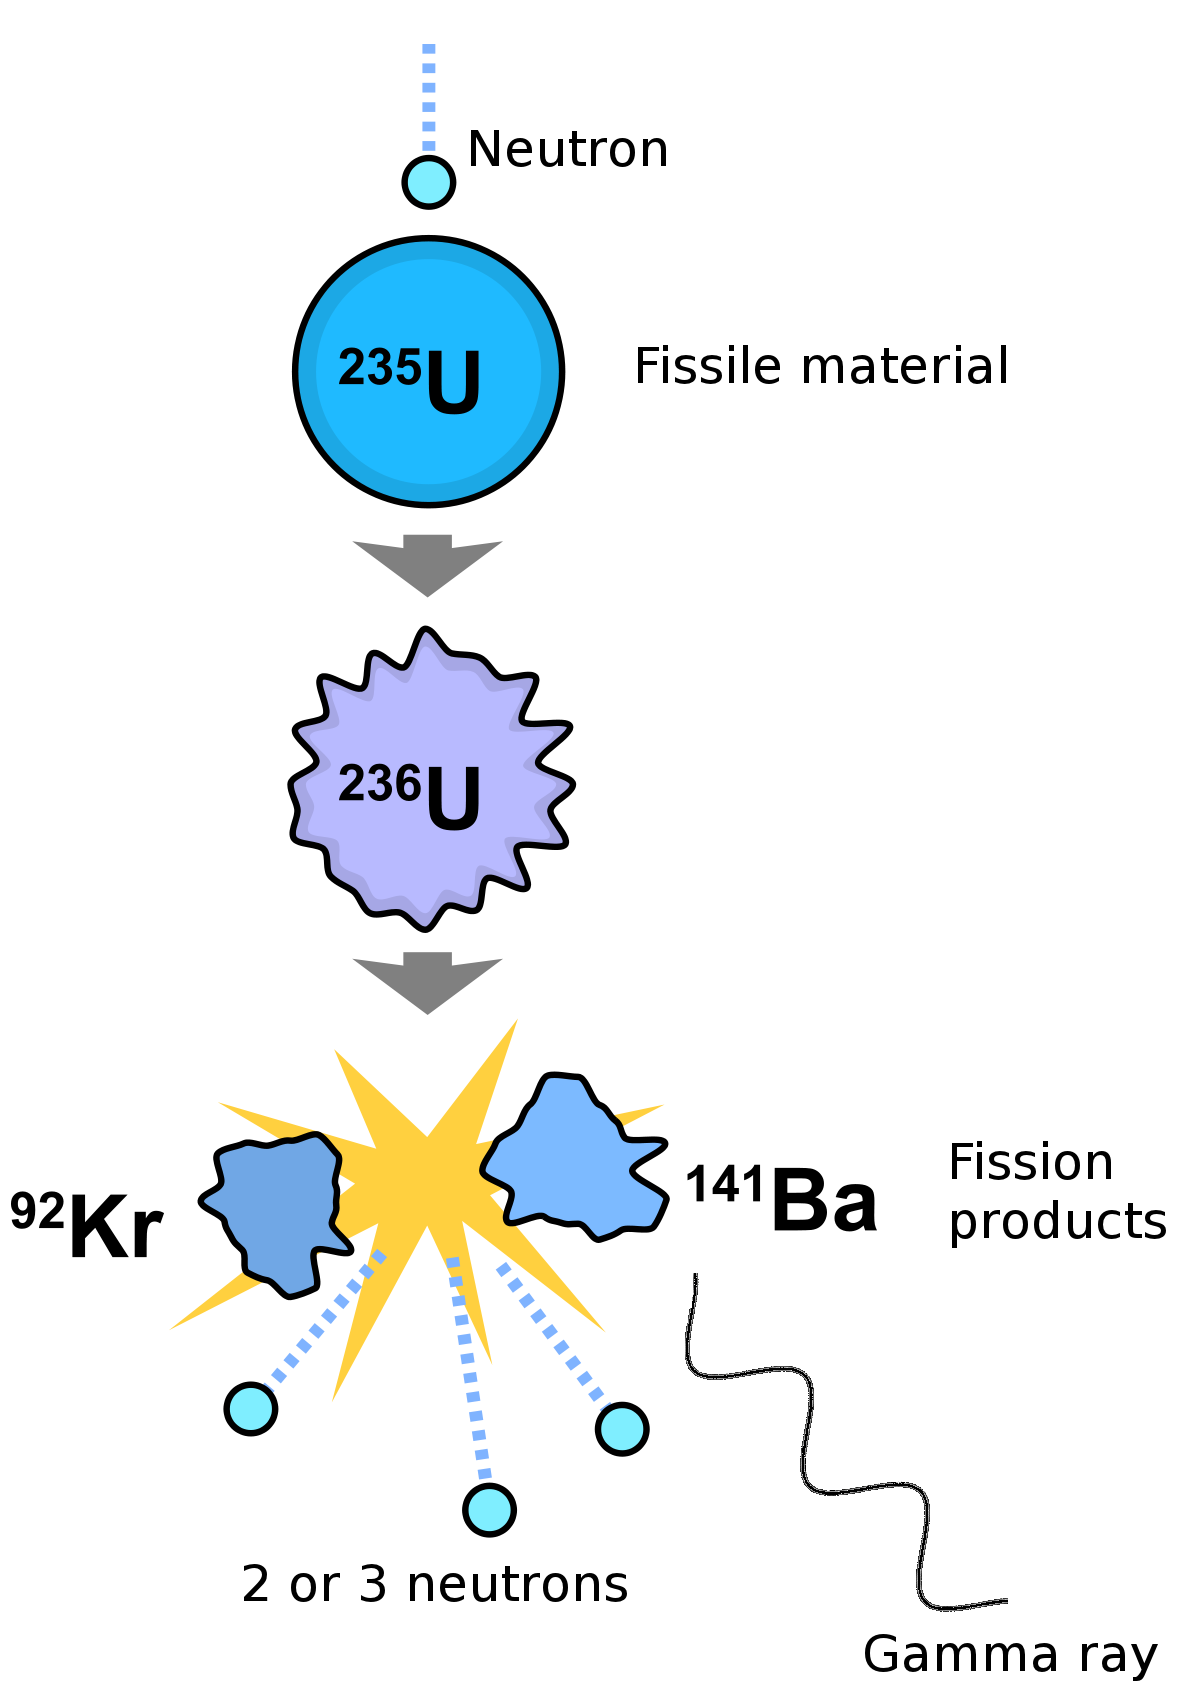
\includegraphics[scale=0.15]{gfx/nuclear-fission.png}
\caption{\label{fig:nuclear-fission}A fission reaction}
\end{figure}
%%%%%%%%%%%%%%%%%%%%%%%%%%%%%%%%%%%%%%%%%%%%5
\part{Appendices}
\begin{appendices}
\chapter{1st Appendix}

\chapter{{2nd Appendix}}


\end{appendices}

\begin{singlespace}
%\fancyhead[LO,LE]{\hfill\raggedleft\emph{References}\hfill\small\thepage\\\quad\\}
    \bibliography{bib}
\bibliographystyle{ieeetr}

%\fancyhead[LO,LE]{\hfill\raggedleft\emph{References}\hfill\small\thepage\\\quad\\}
    %\end{footnotesize}
    \end{singlespace}
%%\bibliographystyle{ieeetr}
%%\bibliography{bib}
\chapter*{{Figure citations}}
%\fancyhead[LO,LE]{\emph{\\\hrule\quad\\\hfill Figure citations}\quad{\bf $|$}\quad\small\bf\thepage}
\fancyhead[LO,LE]{\vspace*{1mm}{\textbf{\quad\\\hfill \small{Figure citations\quad}}{\bf/}}\quad\small\bf\thepage}

\addcontentsline{toc}{chapter}{{Figure citations}}
\doublespacing
\begin{enumerate}
\item {\bf {\Vref{fig:hw-vs-sw}}}\\\url{www.developergeeks.com/article/60/software-reliability-engineering}\\
Author: Brad Stewart (used with permission).
\item {\bf {\Vref{fig:minefield}}}\\\url{http://web.cecs.pdx.edu/~hamlet/pnsqcintro.pdf}\\
Author: Dick Hamlet (used with permission).
\item {\bf {\Vref{fig:nuclear-fission}}}\\
\url{http://en.wikipedia.org/wiki/File:Nuclear_fission.svg}\\(a free image in public domain).
\item {\bf {\Vref{fig:A-typical-sodium-cooled-fast-reactor}}}\\ \url{en.wikipedia.org/wiki/File:Sodium-Cooled_Fast_Reactor_Schemata.svg}\\(a free image in public domain).

\item {\bf {\Vref{fig:sgtld}}}\\Reference: \cite{sgtld-image}\\
Authors: S. Kishore \emph{et al.} (used with permission).
\item {\bf {\Vref{fig:sgdhr}}}\\Reference: \cite{sgdhr-image}\\
Authors: Baldev Raj and Prabhat Kumar (used with permission).
\item {\bf {\Vref{fig:ga}}}\\\url{http://commons.wikimedia.org/wiki/File:Crossover_genes.svg}\\(a free image in public domain).
\end{enumerate}
\end{document}
